In Section \ref{section:MLE} it was shown that the MLE estimate leads to overfitting the parameters if the sample dataset is not a good representation of the population. The MAP estimate overcomes this problem by introducing a prior distribution $P(\theta)$ over the parameter $\theta$. The prior distribution is choosen such that, it has simple interpretation and useful analytical properties. The posterior distribution is proportional to the product of liklihood and prior. If the posterior and prior have same functional form then they are know as conjugate pairs. 

\subsection{Beta distribution}
The beta distribution is a continuos distribution in the interval $[0,1]$ parameterized by two positive shape parameters $a,b$.
\begin{equation}
Beta(\theta|a,b) = \frac{\Gamma(a+b)}{\Gamma(a) \Gamma(b)} \cdot \theta^{a-1} (1-\theta)^{b-1}
\end{equation}
The parameters $a$ and $b$ are also called hyperparameters because they control the distribution of the $\theta$ parameter. The varaince of the beta distribution is governed by the value of the hyperparameters as illustrated in Fig  The beta distribution has similar form as the binomial distribution.  The liklihood function in case of a dataset sampled from a binary random variable takes the form $\theta^{l}(1-\theta)^{m}$. By using the beta distribution as prior, the posterior can then be calulated using the Baye's rule in \ref{equ:bayes}.
\begin{figure}
\begin{center}
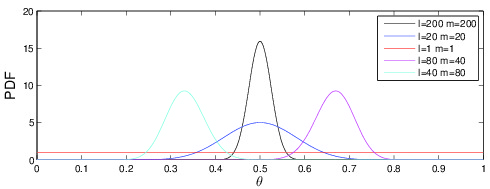
\includegraphics{betaDistribution.jpg}
\caption{Beta Distribution: Depicts the variance of beta distribution for various hyperparameters}
\end{center}
\end{figure}

\begin{equation}
\label{eqn:beta}
posterior(\theta|l,m,a,b) = \frac{\Gamma(a+b+l+m)}{\Gamma(a+l) \Gamma(b+m)} \theta^{a+l-1} (1-\theta)^{b+m-1} = Beta(\theta|a+l,b+m) 
\end{equation}

As seen from Eq. \ref{eqn:beta}, the posterior distribution takes the form of the beta distribution. 

\subsection{Dirichlet distribution}
In case of a Multinomial liklihood function, the beta distribution can be generalized from 2 to K dimensions.
\begin{equation}
Dir(\vec{\theta}|\vec{\alpha}) = \frac{\Gamma(\sum_{k=1}^{K}\alpha_{k})}{\prod_{k=1}^{K}\Gamma(\alpha_{k})}\prod_{k=1}^{K}\theta_{k}
\end{equation}
Similar to the Beta distribution, the posterior distribution in case of Multinomial liklihood function can be shown to the take form of a Dirichlet distribution.